\hypertarget{section-deployment-view}{%
\section{Deployment View}\label{section-deployment-view}}


\begin{figure}
\centering
    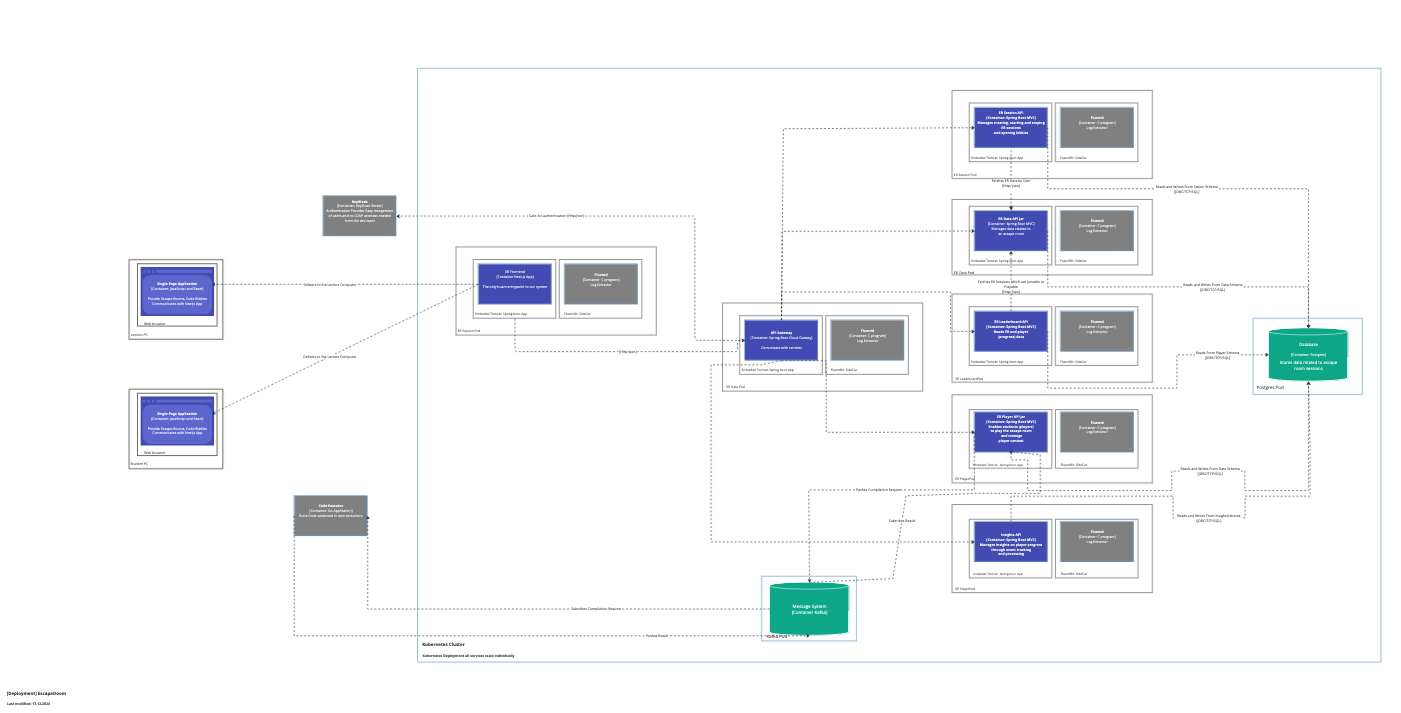
\includegraphics[width=1\linewidth, angle=90]{Deployment.png} % Rotate by 90 degrees
    \caption{Deployment View}
    \label{fig:deployment-view}
\end{figure}

\subsection{Service Deployment Overview}
The system has already been thoroughly described in terms of its building blocks, detailing the components the application consists of. Therefore, the explanation of individual services in this section will be presented generically.

Each service is deployed on the Kubernetes cluster as follows:
\begin{itemize}
    \item A service is deployed within a Kubernetes \textbf{Pod}, which contains:
    \begin{itemize}
        \item A container running the application packaged as a \texttt{.jar} file.
        \item A sidecar container with \textbf{Fluentd} for centralized logging. Fluentd collects logs and pushes them to a centralized log management service.
    \end{itemize}
\end{itemize}

\hypertarget{_infrastructure_level_1}{%
\subsection{Infrastructure Level 1}\label{_infrastructure_level_1}}
Given the use of Kubernetes as the deployment platform, hardware is abstracted and considered a given. Instead, the focus is on the abstractions and capabilities provided by Kubernetes.

\paragraph{Kubernetes Cluster}  
All services, including the frontend and API Gateway, are deployed in a single Kubernetes cluster. Scaling is managed dynamically using the Kubernetes \textbf{Metrics Server}, enabling horizontal scaling based on resource utilization metrics.

\paragraph{Stateful Components}  
\begin{itemize}
    \item \textbf{PostgreSQL and Kafka:} Both stateful components are planned to be deployed within the same cluster (referred to as the "ER cluster"). However, they are designed to be flexible and could also reside outside the cluster if necessary.
    \item \textbf{Code Executor:} For security reasons, the Code Executor is hosted on a restricted platform isolated from the ER cluster to minimize potential vulnerabilities.
\end{itemize}

\paragraph{External Dependencies}  
\begin{itemize}
    \item \textbf{Keycloak:} The Keycloak server is hosted within the customer's domain and is not directly managed by the development team. The configuration of the Keycloak server is coordinated with the responsible administrators through scheduled meetings.
\end{itemize}

\subsection{Keycloak Configuration Deployment}
To roll out the Keycloak configuration, the team uses the following approach:
\begin{itemize}
    \item Configuration files are managed as part of the system's infrastructure-as-code repository.
    \item Scripts or automation tools (e.g., \texttt{kcadm.sh} or custom APIs) are utilized to apply the configurations.
    \item Meetings are arranged with the Keycloak administrators to ensure proper alignment and to verify that the configurations meet the customer's requirements.
\end{itemize}